
\sloppy
\begin{center}{\fontsize{16pt}{16pt}\selectfont \textbf{Python Functions} \\}\end{center} \par
\vspace{12pt}
 \section{Python Functions}
\noindent 
 \hspace*{0.5in} Fungsi adalah blok kode terorganisir dan dapat digunakan kembali yang digunakan untuk melakukan tindakan tunggal dan terkait. Fungsi menyediakan modularitas yang lebih baik untuk aplikasi Anda dan tingkat penggunaan kode yang tinggi. Seperti yang sudah Anda ketahui, Python memberi Anda banyak fungsi built-in seperti cetak (), dll. Tetapi Anda juga dapat membuat fungsi Anda sendiri. Fungsi ini disebut fungsi yang ditentukan pengguna. \par
\vspace{12pt}
\noindent 
\begin{itemize}
	\item Defining a Function 
\end{itemize}
\noindent 
Anda dapat menentukan fungsi untuk menyediakan fungsionalitas yang dibutuhkan.\par
\vspace{\baselineskip}

\begin{itemize}
	\item Built-in Functions
\end{itemize}

\begin{figure}[ht]
	\centerline{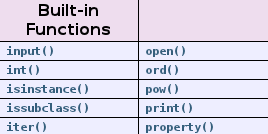
\includegraphics[width=0.70\textwidth]{figures/Functions}}
	\caption{Built-in Functions}
	\label{Built-in Functions}
\end{figure}


\vspace{\baselineskip}
Berikut adalah aturan sederhana untuk mendefinisikan fungsi dengan Python.\par
\vspace{\baselineskip}
\noindent 
 $ \bullet $ Blok fungsi dimulai dari kata kunci diikuti oleh nama fungsi dan tanda kurung (()). \par
 \vspace{\baselineskip}
\noindent 
 $ \bullet $ Setiap parameter masukan atau argumen harus ditempatkan di dalam tanda kurung ini. Anda juga dapat menentukan parameter di dalam tanda kurung ini. \par
 \vspace{\baselineskip}
\noindent 
 $ \bullet $ Pernyataan fungsi pertama dapat berupa pernyataan opsional - string dokumentasi fungsi atau docstring. \par
 \vspace{\baselineskip}
\noindent 
 $ \bullet $ Blok kode dalam setiap fungsi dimulai dengan titik dua (:) dan indentasi. \par
 \vspace{\baselineskip}
\noindent 
 $ \bullet $ Pernyataan kembali [ekspresi] keluar dari sebuah fungsi, secara opsional menyampaikan kembali ekspresi ke pemanggil. Pernyataan pengembalian tanpa argumen sama dengan return None. \par
\vspace{12pt}
\vspace{\baselineskip}
\noindent 
Syntax \par
\begin{verbatim}
def functionname( parameters ): \par
"function_docstring"
function_suite
return [expression]
\end{verbatim}

\vspace{\baselineskip}
\noindent 
Secara default, parameter memiliki perilaku posisi dan Anda perlu memberi tahu mereka dengan urutan yang sama seperti yang ditetapkan. \par
\vspace{12pt}
\vspace{\baselineskip}
\vspace{12pt}
\noindent 
Example \par
\vspace{\baselineskip}
\noindent 
Fungsi berikut mengambil string sebagai parameter masukan dan mencetaknya di layar standar. \par

\begin{verbatim}
def printme( str ): 
"This prints a passed string into this function" 
print str 
return 
\end{verbatim}

\vspace{\baselineskip}
\noindent 
\begin{itemize}
	\item Calling a Function 
\end{itemize}
\noindent 
Mendefinisikan sebuah fungsi hanya memberinya sebuah nama, menentukan parameter yang akan disertakan dalam fungsi dan menyusun blok kode. Setelah struktur dasar fungsi selesai, Anda dapat menjalankannya dengan memanggilnya dari fungsi lain atau langsung dari prompt Python. Berikut adalah contoh untuk memanggil fungsi printme () - \par
\vspace{\baselineskip}
\noindent 
 \hspace*{0.5in}  $  \#  $!/usr/bin/python \par
\vspace{12pt}
\noindent 
 \hspace*{0.5in}  $  \#  $ Function definition is here \par
\noindent 
 \hspace*{0.5in} def printme( str ): \par
 \vspace{\baselineskip}
\noindent 
~~  \hspace*{0.5in}  "This prints a passed string into this function" \par
\noindent 
~~  \hspace*{0.5in} print str \par
\noindent 
~~  \hspace*{0.5in} return; \par
\vspace{12pt}
\noindent 
 \hspace*{0.5in}  $  \#  $ Now you can call printme function \par
\noindent 
 \hspace*{0.5in} printme("I'm first call to user defined function!") \par
\noindent 
 \hspace*{0.5in} printme("Again second call to the same function") \par
 \vspace{\baselineskip}
\noindent 
Bila kode diatas dieksekusi, maka menghasilkan hasil sebagai berikut - \par
\noindent 
 \hspace*{0.5in} I'm first call to user defined function! \par
\noindent 
 \hspace*{0.5in} Again second call to the same function \par
\vspace{12pt}
\vspace{\baselineskip}
\noindent 
Pass by reference vs value \par
\noindent 
Semua parameter (argumen) dalam bahasa Python dilewatkan dengan referensi. Ini berarti jika Anda mengubah parameter yang mengacu pada suatu fungsi, perubahan tersebut juga mencerminkan kembali fungsi pemanggilan. Sebagai contoh - \par
\vspace{\baselineskip}
\noindent 
 \hspace*{0.5in}  $  \#  $!/usr/bin/python \par
\vspace{12pt}
\noindent 
 \hspace*{0.5in}  $  \#  $ Function definition is here \par
\noindent 
 \hspace*{0.5in} def changeme( mylist ): \par
\noindent 
 \hspace*{0.5in} ~~ "This changes a passed list into this function" \par
\noindent 
~~  \hspace*{0.5in}mylist.append([1,2,3,4]); \par
\noindent 
~~  \hspace*{0.5in} print "Values inside the function: ", mylist \par
\noindent 
~~  \hspace*{0.5in} return \par
\noindent 
 \hspace*{0.5in} \vspace{12pt}
 \vspace{\baselineskip}
\noindent 
 \hspace*{0.5in}  $  \#  $ Now you can call changeme function \par
\noindent 
 \hspace*{0.5in} mylist = [10,20,30]; \par
\noindent 
 \hspace*{0.5in} changeme( mylist ); \par
\noindent 
 \hspace*{0.5in} print "Values outside the function: ", mylist \par
 \vspace{\baselineskip}
\noindent 
Di sini, kita mempertahankan referensi objek yang dilewati dan menambahkan nilai pada objek yang sama. Jadi, ini akan menghasilkan hasil sebagai berikut - \par
\vspace{\baselineskip}
\noindent 
 \hspace*{0.5in} Values~inside the function:  [10, 20, 30, [1, 2, 3, 4]] \par
\noindent 
 \hspace*{0.5in} Values~outside the function:  [10, 20, 30, [1, 2, 3, 4]] \par
\vspace{\baselineskip}
\noindent 
Ada satu contoh lagi di mana argumen dilewatkan melalui referensi dan rujukannya ditimpa di dalam fungsi yang disebut. \par
\vspace{\baselineskip}
\noindent 
 \hspace*{0.5in}  $  \#  $!/usr/bin/python \par
\vspace{12pt}
\noindent 
 \hspace*{0.5in}  $  \#  $ Function definition is here \par
\noindent 
 \hspace*{0.5in} def changeme( mylist ): \par
\vspace{\baselineskip}
\noindent 
 \hspace*{0.5in} ~~ "This changes a passed list into this function" \par
\noindent 
 \hspace*{0.5in} ~~ mylist = [1,2,3,4];  $  \#  $ This would assig new reference in mylist \par
\noindent 
 \hspace*{0.5in} ~~ print "Values inside the function: ", mylist \par
\noindent 
 \hspace*{0.5in} ~~ return \par
\vspace{12pt}
\noindent 
 \hspace*{0.5in}  $  \#  $ Now you can call changeme function \par
\noindent 
 \hspace*{0.5in} mylist = [10,20,30]; \par
 \vspace{\baselineskip}
\noindent 
 \hspace*{0.5in} changeme( mylist ); \par
\noindent 
 \hspace*{0.5in} print "Values outside the function: ", mylist \par
\vspace{\baselineskip}
\noindent 
Parameter mylist adalah local ke fungsi changeme. Mengubah mylist dalam fungsi tidak mempengaruhi mylist. Fungsi ini tidak menghasilkan apa-apa dan akhirnya ini akan menghasilkan hasil sebagai berikut: \par
\vspace{\baselineskip}
\noindent 
 \hspace*{0.5in} Values~inside the function:  [1, 2, 3, 4] \par
\noindent 
 \hspace*{0.5in} Values~outside the function:  [10, 20, 30] \par
\vspace{12pt}
\noindent 
\begin{itemize}
	\item Function Arguments 
\end{itemize}
\noindent 
Anda dapat memanggil fungsi dengan menggunakan jenis argumen formal berikut: \par
\noindent 
 \hspace*{0.5in}  $ \bullet $ Argumen yang dibutuhkan \par
\noindent 
 \hspace*{0.5in}  $ \bullet $ Argumen kata kunci \par
\noindent 
 \hspace*{0.5in}  $ \bullet $ Argumen baku \par
\noindent 
 \hspace*{0.5in}  $ \bullet $ Argumen panjang variable \par
\vspace{12pt}
\noindent 
\begin{itemize}
	\item Required arguments
\end{itemize}
\noindent 
Argumen yang diperlukan adalah argumen yang diberikan ke sebuah fungsi dalam urutan posisi yang benar. Di sini, jumlah argumen dalam pemanggilan fungsi harus sesuai persis dengan definisi fungsi. Untuk memanggil fungsi printme (), Anda pasti perlu melewati satu argumen, jika tidak maka akan memberikan kesalahan sintaks sebagai berikut - \par
\vspace{\baselineskip}
\noindent 
 \hspace*{0.5in}  $  \#  $!/usr/bin/python \par
\vspace{12pt}
\noindent 
 \hspace*{0.5in}  $  \#  $ Function definition is here \par
\noindent 
 \hspace*{0.5in} def printme( str ): \par
\noindent 
~~  \hspace*{0.5in}  \hspace*{0.5in} "This prints a passed string into this function" \par
\noindent 
~~  \hspace*{0.5in} print str \par
\noindent 
~~  \hspace*{0.5in} return; \par
\vspace{12pt}
\noindent 
 \hspace*{0.5in}  $  \#  $ Now you can call printme function \par
\noindent 
 \hspace*{0.5in} printme() \par
 \vspace{\baselineskip}
\noindent 
Bila kode diatas dieksekusi, maka menghasilkan hasil sebagai berikut: \par
\noindent 
 \hspace*{0.5in} Traceback (most recent call last): \par
\noindent 
 \hspace*{0.5in} ~ File "test.py", line 11, in <module> \par
\noindent 
 \hspace*{0.5in} ~~~ printme(); \par
\noindent 
 \hspace*{0.5in} TypeError: printme() takes exactly 1 argument (0 given) \par
\vspace{12pt}
\noindent 
\begin{itemize}
	\item Keyword arguments 
\end{itemize}
\noindent 
Argumen kata kunci terkait dengan pemanggilan fungsi. Bila Anda menggunakan argumen kata kunci dalam pemanggilan fungsi, penelepon mengidentifikasi argumen berdasarkan nama parameter. Hal ini memungkinkan Anda melewatkan argumen atau menempatkannya agar tidak bermasalah karena penerjemah Python dapat menggunakan kata kunci yang diberikan agar sesuai dengan nilai parameter. Anda juga dapat membuat panggilan kata kunci ke fungsi printme () dengan cara berikut - \par
\vspace{\baselineskip}
\noindent 
 \hspace*{0.5in}  $  \#  $!/usr/bin/python \par
\vspace{12pt}
\noindent 
 \hspace*{0.5in}  $  \#  $ Function definition is here \par
\noindent 
 \hspace*{0.5in} def printme( str ): \par
\noindent 
 \hspace*{0.5in} ~~ "This prints a passed string into this function" \par
\noindent 
 \hspace*{0.5in} ~~ print str \par
\noindent 
 \hspace*{0.5in} ~~ return; \par
\vspace{12pt}
\noindent 
 \hspace*{0.5in}  $  \#  $ Now you can call printme function \par
\noindent 
 \hspace*{0.5in} printme( str = "My string") \par
 \vspace{\baselineskip}
\noindent 
Bila kode diatas dieksekusi, maka menghasilkan hasil sebagai berikut - \par
\noindent 
 \hspace*{0.5in} My string \par
 \vspace{\baselineskip}
\noindent 
Contoh berikut memberikan gambaran yang lebih jelas. Perhatikan bahwa urutan parameter tidak masalah. \par
\noindent 
 \hspace*{0.5in}  $  \#  $!/usr/bin/python \par
\vspace{12pt}
\noindent 
 \hspace*{0.5in}  $  \#  $ Function definition is here \par
\noindent 
 \hspace*{0.5in} def printinfo( name, age ): \par
\noindent 
 \hspace*{0.5in} ~~ "This prints a passed info into this function" \par
\noindent 
 \hspace*{0.5in} ~~ print "Name: ", name \par
\noindent 
 \hspace*{0.5in} ~~ print "Age ", age \par
\noindent 
 \hspace*{0.5in} ~~ return; \par
\vspace{12pt}
\noindent 
 \hspace*{0.5in}  $  \#  $ Now you can call printinfo function \par
\noindent 
 \hspace*{0.5in} printinfo( age=50, name="miki" ) \par
 \vspace{\baselineskip}
\noindent 
Bila kode diatas dieksekusi, maka menghasilkan hasil sebagai berikut - \par
\noindent 
 \hspace*{0.5in} Name:~ miki \par
\noindent 
 \hspace*{0.5in} Age~ 50 \par
\vspace{12pt}
\noindent 
\begin{itemize}
	\item Default arguments
\end{itemize}
\noindent 
Argumen default adalah argumen yang mengasumsikan nilai default jika nilai tidak diberikan dalam pemanggilan fungsi untuk argumen itu. Contoh berikut memberi ide pada argumen default, ini mencetak usia default jika tidak lulus - \par
\noindent 
 \hspace*{0.5in}  $  \#  $!/usr/bin/python \par
\vspace{12pt}
\noindent 
 \hspace*{0.5in}  $  \#  $ Function definition is here \par
\noindent 
 \hspace*{0.5in} def printinfo( name, age = 35 ): \par
\noindent 
 \hspace*{0.5in} ~~ "This prints a passed info into this function" \par
\noindent 
 \hspace*{0.5in} ~~ print "Name: ", name \par
\noindent 
 \hspace*{0.5in} ~~ print "Age ", age \par
\noindent 
 \hspace*{0.5in} ~~ return; \par
\vspace{12pt}
\noindent 
 \hspace*{0.5in}  $  \#  $ Now you can call printinfo function \par
\noindent 
 \hspace*{0.5in} printinfo( age=50, name="miki" ) \par
\noindent 
 \hspace*{0.5in} printinfo( name="miki" ) \par
 \vspace{\baselineskip}
\noindent 
Bila kode diatas dieksekusi, maka menghasilkan hasil sebagai berikut - \par
\noindent 
 \hspace*{0.5in} Name:~ miki \par
\noindent 
 \hspace*{0.5in} Age~ 50 \par
\noindent 
 \hspace*{0.5in} Name:~ miki \par
\noindent 
 \hspace*{0.5in} Age~ 35 \par
\vspace{12pt}
\noindent 
\begin{itemize}
	\item Variable-length arguments 
\end{itemize}
\noindent 
Anda mungkin perlu memproses sebuah fungsi untuk argumen lebih banyak daripada yang Anda tentukan saat menentukan fungsinya. Argumen ini disebut variable-lengtharguments dan tidak disebutkan dalam definisi fungsi, tidak seperti argumen yang dibutuhkan dan standar. \par
\vspace{\baselineskip}
\noindent 
Sintaks untuk fungsi dengan argumen variabel non-kata kunci adalah ini - \par
\vspace{\baselineskip}
\noindent 
 \hspace*{0.5in} def functionname([formal $  \_  $args,] *var $  \_  $args $  \_  $tuple ): \par
\noindent 
 \hspace*{0.5in} ~~ "function $  \_  $docstring" \par
\noindent 
 \hspace*{0.5in} ~~ function $  \_  $suite \par
\noindent 
 \hspace*{0.5in} ~~ return [expression] \par
 \vspace{\baselineskip}
\noindent 
Tanda asterisk (*) ditempatkan sebelum nama variabel yang menyimpan nilai dari semua argumen variabel nonkeyword. Tuple ini tetap kosong jika tidak ada argumen tambahan yang ditentukan selama pemanggilan fungsi. Berikut adalah contoh sederhana - \par
\vspace{\baselineskip}
\noindent 
 \hspace*{0.5in}  $  \#  $!/usr/bin/python \par
\vspace{12pt}
\noindent 
 \hspace*{0.5in}  $  \#  $ Function definition is here \par
\noindent 
 \hspace*{0.5in} def printinfo( arg1, *vartuple ): \par
\vspace{\baselineskip}
\noindent 
 \hspace*{0.5in} ~~ "This prints a variable passed arguments" \par
\noindent 
 \hspace*{0.5in} ~~ print "Output is: " \par
\noindent 
 \hspace*{0.5in} ~~ print arg1 \par
\noindent 
 \hspace*{0.5in} ~~ for var in vartuple: \par
\noindent 
 \hspace*{0.5in} ~~~~~ print var \par
\noindent 
 \hspace*{0.5in} ~~ return; \par
\noindent 
 \hspace*{0.5in} \vspace{12pt}
\noindent 
 \hspace*{0.5in}  $  \#  $ Now you can call printinfo function \par
\noindent 
 \hspace*{0.5in} printinfo( 10 ) \par
\noindent 
 \hspace*{0.5in} printinfo( 70, 60, 50 ) \par
 \vspace{\baselineskip}
\noindent 
Bila kode diatas dieksekusi, maka menghasilkan hasil sebagai berikut - \par
\vspace{\baselineskip}
\vspace{\baselineskip}
\noindent 
 \hspace*{0.5in} Output is: \par
\noindent 
 \hspace*{0.5in} 10 \par
 \vspace{\baselineskip}
\noindent 
 \hspace*{0.5in} Output is: \par
\noindent 
 \hspace*{0.5in} 70 \par
\noindent 
 \hspace*{0.5in} 60 \par
\noindent 
 \hspace*{0.5in} 50 \par
 \vspace{\baselineskip}
\noindent 
\begin{itemize}
	\item The Anonymous Functions
\end{itemize}
\noindent 
Fungsi ini disebut anonim karena tidak dinyatakan secara standar dengan menggunakan kata kunci def. Anda bisa menggunakan kata kunci lambda untuk membuat fungsi anonim yang kecil. \par
\noindent 
$ \bullet $ Bentuk lambda bisa mengambil sejumlah argumen tapi hanya mengembalikan satu nilai dalam bentuk ekspresi. Mereka tidak dapat berisi perintah atau beberapa ekspresi. \par
\noindent 
$ \bullet $ Fungsi anonim tidak bisa menjadi panggilan langsung untuk dicetak karena lambda membutuhkan ekspresi \par
\noindent 
$ \bullet $ Fungsi Lambda memiliki namespace lokal mereka sendiri dan tidak dapat mengakses variabel selain yang ada dalam daftar parameter dan yang ada di namespace global. \par
\noindent 
$ \bullet $ Meskipun tampak bahwa lambda adalah versi satu baris dari sebuah fungsi, mereka tidak setara dengan pernyataan inline di C atau C ++, yang tujuannya adalah dengan melewatkan alokasi stack fungsi selama pemanggilan untuk alasan kinerja. \par
\vspace{12pt}
\vspace{12pt}
\noindent 
Syntax \par
\vspace{\baselineskip}
\noindent 
Sintaks fungsi lambda hanya berisi satu pernyataan, yaitu sebagai berikut - \par
\noindent 
 \hspace*{0.5in} lambda [arg1 [,arg2,.....argn]]:expression \par
\noindent 
Berikut adalah contoh untuk menunjukkan bagaimana lambda bentuk fungsi bekerja - \par
\noindent 
 \hspace*{0.5in}  $  \#  $!/usr/bin/python \par
\vspace{12pt}
\noindent 
 \hspace*{0.5in}  $  \#  $ Function definition is here \par
\noindent 
 \hspace*{0.5in} sum = lambda arg1, arg2: arg1 + arg2; \par
\vspace{12pt}
\noindent 
  \par
\vspace{12pt}
\noindent 
 \hspace*{0.5in}  $  \#  $ Now you can call sum as a function \par
\noindent 
 \hspace*{0.5in} print "Value of total : ", sum( 10, 20 ) \par
\noindent 
 \hspace*{0.5in} print "Value of total : ", sum( 20, 20 ) \par
\vspace{\baselineskip}
\noindent 
Bila kode diatas dieksekusi, maka menghasilkan hasil sebagai berikut - \par
\noindent 
 \hspace*{0.5in} Value~of total :  30 \par
\noindent 
 \hspace*{0.5in} Value~of total :  40 \par
\vspace{12pt}
\noindent 
\begin{itemize}
	\item The return Statement 
\end{itemize}
\noindent 
Pernyataan kembali [ekspresi] keluar dari sebuah fungsi, secara opsional menyampaikan kembali ekspresi ke pemanggil. Pernyataan pengembalian tanpa argumen sama dengan return None. \par
\vspace{\baselineskip}
\noindent 
Semua contoh di atas tidak mengembalikan nilai apapun. Anda bisa mengembalikan nilai dari sebuah fungsi sebagai berikut - \par
\vspace{\baselineskip}
\noindent 
 \hspace*{0.5in}  $  \#  $!/usr/bin/python \par
\vspace{12pt}
\noindent 
 \hspace*{0.5in}  $  \#  $ Function definition is here \par
\noindent 
 \hspace*{0.5in} def sum( arg1, arg2 ): \par
\noindent 
 \hspace*{0.5in} ~~  $  \#  $ Add both the parameters and return them." \par
\noindent 
 \hspace*{0.5in} ~~ total = arg1 + arg2 \par
\noindent 
 \hspace*{0.5in} ~~ print "Inside the function : ", total \par
\noindent 
 \hspace*{0.5in} ~~ return total; \par
\vspace{12pt}
\noindent 
 \hspace*{0.5in}  $  \#  $ Now you can call sum function \par
\noindent 
 \hspace*{0.5in} total = sum( 10, 20 ); \par
\noindent 
 \hspace*{0.5in} print "Outside the function : ", total  \par
 \vspace{\baselineskip}
\noindent 
Bila kode diatas dieksekusi, maka menghasilkan hasil sebagai berikut - \par
\noindent 
 \hspace*{0.5in} Inside~the function :  30 \par
\noindent 
 \hspace*{0.5in} Outside~the function :  30 \par
\noindent 
\subsection{Scope of Variables }
\noindent 
Semua variabel dalam sebuah program mungkin tidak dapat diakses di semua lokasi dalam program tersebut. Ini tergantung di mana Anda telah menyatakan sebuah variabel. \par
\noindent 
Ruang lingkup variabel menentukan bagian dari program di mana Anda dapat mengakses pengenal tertentu. Ada dua lingkup dasar variabel dengan Python - \par
\noindent 
 \hspace*{0.5in}  $ \bullet $ Variabel global \par
\noindent 
 \hspace*{0.5in}  $ \bullet $ Variabel local \par
\vspace{12pt}
\noindent 
\subsection{Global vs. Local variables }
\noindent 
Variabel yang didefinisikan di dalam badan fungsi memiliki lingkup lokal, dan yang didefinisikan di luar memiliki cakupan global. \par
\noindent 
Ini berarti bahwa variabel lokal dapat diakses hanya di dalam fungsi di mana mereka dideklarasikan, sedangkan variabel global dapat diakses di seluruh tubuh program oleh semua fungsi. Saat Anda memanggil fungsi, variabel yang dideklarasikan di dalamnya dibawa ke lingkup. Berikut adalah contoh sederhana - \par
\vspace{\baselineskip}
\noindent 
 \hspace*{0.5in}  $  \#  $!/usr/bin/python \par
\vspace{12pt}
\noindent 
 \hspace*{0.5in} total = 0;  $  \#  $ This is global variable. \par
\noindent 
 \hspace*{0.5in}  $  \#  $ Function definition is here \par
\noindent 
 \hspace*{0.5in} def sum( arg1, arg2 ): \par
 \vspace{\baselineskip}
\noindent 
 \hspace*{0.5in} ~~  $  \#  $ Add both the parameters and return them." \par
\noindent 
 \hspace*{0.5in} ~~ total = arg1 + arg2;  $  \#  $ Here total is local variable. \par
\noindent 
 \hspace*{0.5in} ~~ print "Inside the function local total : ", total \par
\noindent 
 \hspace*{0.5in} ~~ return total; \par
\noindent 
 \hspace*{0.5in} \vspace{12pt}
\noindent 
 \hspace*{0.5in}  $  \#  $ Now you can call sum function \par
\noindent 
 \hspace*{0.5in} sum( 10, 20 ); \par
\noindent 
 \hspace*{0.5in} print "Outside the function global total : ", total  \par
\vspace{\baselineskip}
\noindent 
Bila kode diatas dieksekusi, maka menghasilkan hasil sebagai berikut - \par
\noindent 
 \hspace*{0.5in} Inside~the function local total :  30 \par
\noindent 
 \hspace*{0.5in} Outside~the function global total :  0 \par
 \vspace{\baselineskip}
 \vspace{\baselineskip}
 
 \begin{itemize}
 	\item Python Tuple Functions
 \end{itemize}
 
 \begin{figure}[ht]
 	\centerline{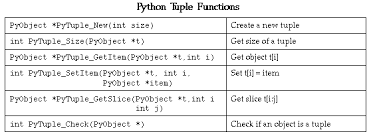
\includegraphics[width=0.70\textwidth]{figures/Functions1}}
 	\caption{Python Tuple Functions}
 	\label{Python Tuple Functions}
 \end{figure}

